% Homepage thumbnail for AFVE-Bench (rendered to images/afve_bench.jpg at 320x320).
%   pdflatex afve_bench_thumb.tex && pdftoppm -jpeg -jpegopt quality=90 -singlefile -scale-to 320 afve_bench_thumb.pdf ../afve_bench
\documentclass[tikz,border=0pt]{standalone}
\usepackage[scaled]{helvet}
\renewcommand{\familydefault}{\sfdefault}
\usetikzlibrary{arrows.meta}
\definecolor{Afill}{HTML}{FBE3C2}\definecolor{Aline}{HTML}{D9902F}
\definecolor{Bfill}{HTML}{DCE8F8}\definecolor{Bline}{HTML}{4A7CC0}
\definecolor{Red}{HTML}{C0392B}\definecolor{Redfill}{HTML}{FBE1DE}
\definecolor{Ink}{HTML}{333333}\definecolor{Bar}{HTML}{C9CED6}
\begin{document}
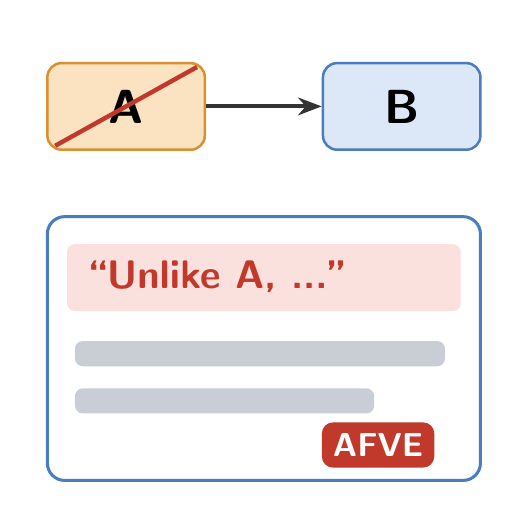
\begin{tikzpicture}[x=1mm,y=1mm,font=\bfseries\color{Ink}]
  \fill[white] (0,0) rectangle (60,60);
  % the user switches from frame A to frame B
  \node[draw=Aline,fill=Afill,rounded corners=1.8mm,line width=0.9pt,minimum width=20mm,minimum height=11mm,font=\bfseries\LARGE] (A) at (12.5,50) {A};
  \node[draw=Bline,fill=Bfill,rounded corners=1.8mm,line width=0.9pt,minimum width=20mm,minimum height=11mm,font=\bfseries\LARGE] (B) at (47.5,50) {B};
  \draw[-{Stealth[length=3mm]},line width=1.4pt,Ink] (A) -- (B);
  \draw[Red,line width=1.6pt] (3.5,45) -- (21.5,55);
  % the revised answer adopts B but still mentions A
  \draw[Bline,line width=1.1pt,fill=white,rounded corners=2.2mm] (2.5,2.5) rectangle (57.5,36);
  \fill[Redfill,rounded corners=1mm] (5,24) rectangle (55,32.5);
  \node[anchor=west,font=\bfseries\Large,text=Red] at (6,28.4) {``Unlike A, ...''};
  \foreach \y/\w in {17/47,11/38} \fill[Bar,rounded corners=1mm] (6,\y) rectangle (6+\w,\y+3.2);
  \node[fill=Red,text=white,rounded corners=1.4mm,font=\bfseries\large,inner sep=1.4mm] at (44.5,7) {AFVE};
\end{tikzpicture}
\end{document}
